% docs/slides/preamble.tex -- 五份 deck 共享
\documentclass[aspectratio=169,11pt]{beamer}

% ==== 中文与字体 ====
\usepackage[UTF8,fontset=none]{ctex}
\usepackage{fontspec}

\IfFontExistsTF{PingFang SC}{%
  \setCJKmainfont{PingFang SC}[BoldFont=PingFang SC,ItalicFont=PingFang SC,AutoFakeSlant=0.15]
  \setCJKsansfont{PingFang SC}[ItalicFont=PingFang SC,AutoFakeSlant=0.15]
  \setCJKmonofont{PingFang SC}
}{%
  \IfFontExistsTF{Source Han Sans SC}{%
    \setCJKmainfont{Source Han Sans SC}
    \setCJKsansfont{Source Han Sans SC}
  }{%
    \IfFontExistsTF{Noto Sans CJK SC}{%
      \setCJKmainfont{Noto Sans CJK SC}
      \setCJKsansfont{Noto Sans CJK SC}
    }{%
      \setCJKmainfont{Heiti SC}
      \setCJKsansfont{Heiti SC}
    }
  }
}

\IfFontExistsTF{Helvetica Neue}{\setmainfont{Helvetica Neue}}{%
  \IfFontExistsTF{Inter}{\setmainfont{Inter}}{}}
\IfFontExistsTF{JetBrains Mono}{\setmonofont{JetBrains Mono}[Scale=0.85]}%
  {\setmonofont{Menlo}[Scale=0.85]}

% ==== 颜色 ====
\usepackage{xcolor}
\definecolor{cMain}{HTML}{1F4E79}
\definecolor{cAccent}{HTML}{E07A1F}
\definecolor{cGray}{HTML}{595959}
\definecolor{cMute}{HTML}{F4F4F4}
\definecolor{cOK}{HTML}{2E7D32}
\definecolor{cBad}{HTML}{B23A3A}
\definecolor{cWarn}{HTML}{C8A300}

% ==== 主题 ====
\usepackage{tcolorbox}
\usetheme{metropolis}
\metroset{progressbar=frametitle,numbering=fraction,block=fill}
\setbeamercolor{frametitle}{bg=cMain,fg=white}
\setbeamercolor{progress bar}{fg=cAccent,bg=cMute}
\setbeamercolor{alerted text}{fg=cAccent}
\setbeamercolor{title}{fg=cMain}

% metropolis 默认尝试 Fira Sans，未安装时 fallback 到 Latin Modern Sans。
% 这里在主题加载后显式覆盖，强制使用 macOS 上一定存在的 Helvetica Neue，
% 跟中文 PingFang 风格一致；找不到则按顺序尝试 Inter / Arial。
\IfFontExistsTF{Helvetica Neue}{%
  \setsansfont{Helvetica Neue}%
}{%
  \IfFontExistsTF{Inter}{\setsansfont{Inter}}{%
    \IfFontExistsTF{Arial}{\setsansfont{Arial}}{}}%
}

% ==== TikZ ====
\usepackage{tikz}
\usetikzlibrary{positioning,arrows.meta,fit,shapes.geometric,calc,%
  decorations.pathmorphing,backgrounds}

\tikzset{
  node-box/.style={draw=cMain,thick,rounded corners=2pt,
    minimum height=8mm,minimum width=18mm,align=center,font=\small},
  node-state/.style={draw=cMain,thick,circle,minimum size=14mm,
    align=center,font=\small},
  node-ok/.style={draw=cOK,thick,fill=cOK!10},
  node-warn/.style={draw=cWarn,thick,fill=cWarn!15},
  node-bad/.style={draw=cBad,thick,fill=cBad!10},
  % 色盲友好的状态机三态：蓝 (正常/Closed) / 橙 (告警/Open) / 灰 (中间/HalfOpen)
  % 避免 red-green 二元区分，改用 hue + lightness 双通道。
  node-state-normal/.style={draw=cMain,thick,fill=cMain!12},
  node-state-alert/.style={draw=cAccent,thick,fill=cAccent!18},
  node-state-transition/.style={draw=cGray,thick,fill=cGray!18},
  arrow/.style={-{Stealth[length=2mm]},thick,draw=cMain},
  arrow-async/.style={-{Stealth[length=2mm]},thick,dashed,draw=cGray},
  arrow-bad/.style={-{Stealth[length=2mm]},thick,draw=cBad},
  arrow-alert/.style={-{Stealth[length=2mm]},thick,draw=cAccent},
  lifeline/.style={dashed,thick,draw=cGray},
}

% ==== 代码 ====
\usepackage{listings}
\lstdefinelanguage{Go}{
  morekeywords={break,case,chan,const,continue,default,defer,else,
    fallthrough,for,func,go,goto,if,import,interface,map,package,range,
    return,select,struct,switch,type,var,nil,true,false,iota},
  morekeywords=[2]{string,int,int64,uint,uint64,bool,byte,error,context},
  sensitive=true,
  morecomment=[l]//,morecomment=[s]{/*}{*/},
  morestring=[b]",morestring=[b]`,
}
\lstdefinelanguage{LuaRedis}{
  morekeywords={and,break,do,else,elseif,end,false,for,function,if,in,
    local,nil,not,or,repeat,return,then,true,until,while},
  morekeywords=[2]{redis,call,KEYS,ARGV,tonumber,HGET,HSET,GET,SET,
    DECR,DECRBY,INCR,INCRBY,EXPIRE,PEXPIRE,ZADD,ZCARD,ZREMRANGEBYSCORE,
    EVAL,EVALSHA},
  sensitive=true,
  morecomment=[l]{--},
  morestring=[b]",morestring=[b]',
}

\lstdefinestyle{base}{
  basicstyle=\ttfamily\scriptsize,
  numbers=left,numberstyle=\tiny\color{cGray},
  keywordstyle=\color{cMain}\bfseries,
  keywordstyle=[2]\color{cAccent},
  stringstyle=\color{cOK},
  commentstyle=\color{cGray}\itshape,
  backgroundcolor=\color{cMute},
  frame=single,framerule=0pt,
  showstringspaces=false,
  breaklines=true,
  tabsize=2,
  columns=fullflexible,
}
\lstset{style=base}

% ==== 三线表与附录页码 ====
\usepackage{booktabs}
\usepackage{appendixnumberbeamer}

% ==== 页脚来源标注 ====
\newcommand{\srcnote}[1]{{\color{cGray}\scriptsize\itshape #1}}

% 关键论点框
\newcommand{\keypoint}[1]{%
  \begin{tcolorbox}[colback=cMute,colframe=cMain,boxrule=0.5pt,arc=2pt]%
  #1\end{tcolorbox}}


\title{限流与熔断}
\subtitle{令牌桶、滑动窗口、三态熔断器一次性梳清}
\author{gomall · 后端实战}
\date{}

\begin{document}

\maketitle

\begin{frame}{今日大纲}
\tableofcontents
\end{frame}

% ============== 1. 为什么限流 ==============
\section{为什么要限流}

\begin{frame}{误区："我能扛 5w RPS，不需要限流"}
\begin{itemize}
  \item 单机基线 64{,}254 RPS（\texttt{/ping}），听起来很安全。
  \item 但下游 DB / 第三方服务 / 风控 不一定扛得住。
  \item 限流是\textbf{保护下游}，不是保护自己。
\end{itemize}
\srcnote{stressTest/REPORT.md \S 链路压测表 第 1 行 64{,}254 RPS}
\end{frame}

\begin{frame}{限流的四个目的}
\begin{tikzpicture}[node distance=8mm and 14mm]
  \node[node-box,node-warn] (gw) {网关};
  \node[node-box,above right=of gw] (vip) {VIP 用户};
  \node[node-box,right=of gw] (free) {普通用户};
  \node[node-box,below right=of gw,node-bad] (bot) {爬虫/滥用};
  \node[node-box,right=22mm of free,node-ok] (svc) {Service};
  \draw[arrow] (vip) -- (gw);
  \draw[arrow] (free) -- (gw);
  \draw[arrow-bad] (bot) -- (gw);
  \draw[arrow] (gw) -- node[above,font=\tiny]{配额}(svc);
\end{tikzpicture}
\vspace{2mm}
\begin{enumerate}
  \item 隔离故障爆炸半径。
  \item 保护下游容量。
  \item 用户分级 (VIP $\gg$ 普通)。
  \item 防滥用 / 防爬虫。
\end{enumerate}
\end{frame}

% ============== 2. 三种算法对比 ==============
\section{三种限流算法}

\begin{frame}{三种算法对比}
\begin{tabular}{@{}llll@{}}
\toprule
算法 & 精度 & 突发 & 复杂度 \\
\midrule
固定窗口计数器 & 低 (临界突刺) & 不支持 & 低 \\
令牌桶 & 中 & \textbf{支持 burst} & 低 \\
滑动窗口 (ZSet) & 高 & 支持 & 中 \\
\bottomrule
\end{tabular}
\vspace{3mm}
\small 选型：单机用令牌桶 (\texttt{golang.org/x/time/rate})；分布式用 Redis 滑动窗口。
\srcnote{docs/blog/05-ratelimit-circuit-breaker.md \S 三种限流算法}
\end{frame}

\begin{frame}{计数器临界突刺}
\begin{tikzpicture}
  \draw[arrow] (0,0) -- (9,0);
  \draw[cGray] (1,-0.1) -- (1,0.1); \node[font=\tiny,below] at (1,-0.1) {1s};
  \draw[cGray] (4,-0.1) -- (4,0.1); \node[font=\tiny,below] at (4,-0.1) {2s};
  \draw[cGray] (7,-0.1) -- (7,0.1); \node[font=\tiny,below] at (7,-0.1) {3s};
  \node[node-box,minimum width=20mm,minimum height=8mm] at (2.5,0.8) {Window A};
  \node[node-box,minimum width=20mm,minimum height=8mm] at (5.5,0.8) {Window B};
  \node[font=\small,text=cBad] at (4,1.8) {1.99s 放 100 + 2.01s 放 100 = 0.02s 内放 200};
  \draw[arrow-bad,thick] (3.85,1.5) -- (3.85,0.4);
  \draw[arrow-bad,thick] (4.15,1.5) -- (4.15,0.4);
\end{tikzpicture}
\vspace{2mm}
\small 固定窗口在边界上没有连续性，突发可以达到 2 倍阈值。
\end{frame}

\begin{frame}{令牌桶：burst + 速率}
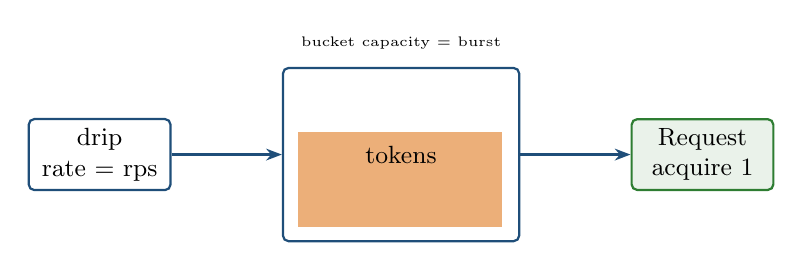
\begin{tikzpicture}[node distance=8mm and 14mm]
  \node[draw=cMain,thick,rounded corners=2pt,minimum width=30mm,minimum height=22mm] (bucket) {};
  \node[font=\tiny] at (bucket.north) [above=1mm] {bucket capacity = burst};
  \fill[cAccent!60] (bucket.south west) ++(2mm,2mm) rectangle ++(26mm,12mm);
  \node[font=\small] at (bucket.center) {tokens};
  \node[node-box,left=of bucket] (drip) {drip\\rate = rps};
  \node[node-box,right=of bucket,node-ok] (req) {Request\\acquire 1};
  \draw[arrow] (drip) -- (bucket);
  \draw[arrow] (bucket) -- (req);
\end{tikzpicture}
\vspace{2mm}
\small 令牌按速率滴入，请求消耗令牌 —— 短时突发允许 burst 个，长时受 rps 限制。
\end{frame}

\begin{frame}[fragile]{单机令牌桶中间件}
\begin{lstlisting}[language=Go,firstnumber=22,
  caption={\srcnote{middleware/ratelimit.go:22--49}}]
func TokenBucket(rps rate.Limit, burst int) gin.HandlerFunc {
    var mu sync.Mutex
    limiters := make(map[string]*rate.Limiter)
    get := func(ip string) *rate.Limiter {
        mu.Lock(); defer mu.Unlock()
        l, ok := limiters[ip]
        if !ok { l = rate.NewLimiter(rps, burst); limiters[ip] = l }
        return l
    }
    return func(c *gin.Context) {
        if !get(c.ClientIP()).Allow() {
            c.JSON(200, gin.H{"status": e.ErrRateLimitExceeded, ...})
            c.Abort(); return
        }
        c.Next()
    }
}
\end{lstlisting}
\end{frame}

% ============== 3. 分布式滑动窗口 ==============
\section{分布式滑动窗口}

\begin{frame}{单机桶的硬伤}
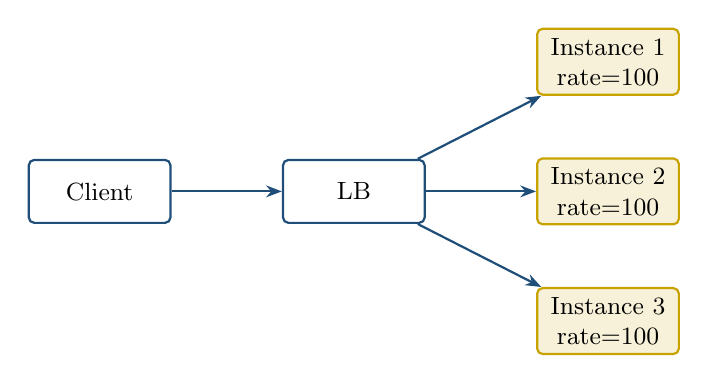
\begin{tikzpicture}[node distance=8mm and 14mm]
  \node[node-box] (cli) {Client};
  \node[node-box,right=of cli] (lb) {LB};
  \node[node-box,above right=of lb,node-warn] (i1) {Instance 1\\rate=100};
  \node[node-box,right=of lb,node-warn] (i2) {Instance 2\\rate=100};
  \node[node-box,below right=of lb,node-warn] (i3) {Instance 3\\rate=100};
  \draw[arrow] (cli) -- (lb);
  \draw[arrow] (lb) -- (i1);
  \draw[arrow] (lb) -- (i2);
  \draw[arrow] (lb) -- (i3);
\end{tikzpicture}
\vspace{2mm}
\small 3 个实例各自限 100 RPS $\to$ 全局放过 300 RPS。\\
单机算法无法对外承诺全局阈值，必须把状态外置到 Redis。
\end{frame}

\begin{frame}{ZSet 滑动窗口设计}
\begin{tikzpicture}[node distance=8mm]
  \node[draw=cMain,thick,rounded corners=2pt,minimum width=80mm,minimum height=14mm] (zset) {};
  \node[font=\tiny] at (zset.north) [above=1mm] {ZSet: \texttt{rl:scope:user}};
  \node[font=\scriptsize,text=cMain] at ($(zset.west)+(8mm,2mm)$) {member: req\_id};
  \node[font=\scriptsize,text=cMain] at ($(zset.west)+(8mm,-2mm)$) {score: ts (ms)};
  \draw[cGray] ($(zset.south)+(0,-3mm)$) -- ($(zset.south)+(80mm,0)+(0,-3mm)$);
  \node[font=\tiny,text=cGray,below=4mm of zset.south] {ZREMRANGEBYSCORE 删除 < now-window 的；ZCARD 计数；ZADD 入新点};
\end{tikzpicture}
\vspace{2mm}
\begin{itemize}
  \item ZSet 按 score (时间戳) 排序，天然支持区间删除。
  \item ZCARD O(1) 拿当前窗口内请求数。
  \item 比 List 灵活：精确删除过期点而不是按头尾。
\end{itemize}
\end{frame}

\begin{frame}[fragile]{滑动窗口 Lua 脚本}
\begin{lstlisting}[language=LuaRedis,firstnumber=18,
  caption={\srcnote{repository/cache/ratelimit.go:18--34}}]
local key       = KEYS[1]
local window_ms = tonumber(ARGV[1])
local limit     = tonumber(ARGV[2])
local now_ms    = tonumber(ARGV[3])
local member    = ARGV[4]

redis.call('ZREMRANGEBYSCORE', key, 0, now_ms - window_ms)
local count = redis.call('ZCARD', key)
if count >= limit then
    return {0, count}
end

redis.call('ZADD', key, now_ms, member)
redis.call('PEXPIRE', key, window_ms)
return {1, count + 1}
\end{lstlisting}
\end{frame}

\begin{frame}[fragile]{中间件：scope + ByUser}
\begin{lstlisting}[language=Go,firstnumber=59,
  caption={\srcnote{middleware/ratelimit.go:59--106}}]
func SlidingWindow(opt SlidingWindowOption) gin.HandlerFunc {
    return func(c *gin.Context) {
        identifier := c.ClientIP()
        if opt.ByUser {
            if u, err := ctl.GetUserInfo(c.Request.Context()); err == nil {
                identifier = formatUint(u.Id)
            }
        }
        key := cache.RateLimitKey(opt.Scope, identifier)
        nowMS := time.Now().UnixMilli()
        member := formatInt(nowMS) + "-" + randomHex()
        allowed, _, _ := cache.SlidingWindowAllow(c.Request.Context(),
            key, opt.Window.Milliseconds(), opt.Limit, nowMS, member)
        if !allowed { c.JSON(200, gin.H{"status": e.ErrRateLimitExceeded}); c.Abort(); return }
        c.Next()
    }
}
\end{lstlisting}
\end{frame}

\begin{frame}{压测：精度误差 < 3\%}
\textbf{场景}：30 VU $\times$ 15s 打 \texttt{/skill\_product/skill}，\texttt{Limit=3 Window=1s ByUser=true}。

\vspace{3mm}
\begin{tabular}{@{}lr@{}}
\toprule
指标 & 数值 \\
\midrule
被限流 (status=70001) & \textbf{781{,}624} \\
通过 & \textbf{46} \\
期望 (15s $\times$ 3/s) & 45 \\
误差 & $\approx$ 2.2\% \\
\bottomrule
\end{tabular}
\vspace{2mm}
\srcnote{stressTest/REPORT.md \S 5. 限流中间件}
\end{frame}

\begin{frame}{ZSet 性能基线}
\begin{itemize}
  \item ZADD / ZREMRANGEBYSCORE / ZCARD 都是 O(logN)，N = 当前窗口内请求数。
  \item 1000 RPS 窗口 N $\approx$ 1000，单 op $<$ 10$\mu$s。
  \item Redis 单节点 10w QPS 完全扛得住分布式限流场景。
\end{itemize}
\srcnote{stressTest/REPORT.md \S 链路压测 第 7 行：秒杀 + 限流 52{,}082 RPS / p95 1.24ms}
\end{frame}

% ============== 4. 熔断 ==============
\section{三态熔断器}

\begin{frame}{熔断的痛点：goroutine 堆积}
\begin{tikzpicture}[node distance=8mm and 16mm]
  \node[node-box] (app) {App};
  \node[node-box,right=of app,node-bad] (down) {下游\\30s 超时};
  \node[node-box,below=of app,node-warn] (gor) {3000 个 goroutine\\堆积等下游};
  \draw[arrow] (app) -- (down);
  \draw[arrow-bad] (app) -- (gor);
\end{tikzpicture}
\vspace{2mm}
\small 下游变慢但不报错时最危险：上游 goroutine 持续堆积 $\to$ 内存爆 $\to$ 进程崩。\\
熔断的核心：\textbf{下游已经病了，就别再喂请求过去}。
\end{frame}

\begin{frame}{三态机：Closed / Open / HalfOpen}
\begin{tikzpicture}[node distance=26mm]
  \node[node-state,node-state-normal] (cl) {Closed};
  \node[node-state,node-state-alert,right=of cl] (op) {Open};
  \node[node-state,node-state-transition,below=20mm of op] (ho) {HalfOpen};

  \draw[arrow-alert] (cl) -- node[above,font=\tiny]{failures $\geq$ threshold} (op);
  \draw[arrow] (op) -- node[right,font=\tiny]{wait OpenTimeout} (ho);
  \draw[arrow,bend left=20] (ho) to node[right,font=\tiny]{探测全成功} (cl);
  \draw[arrow-alert,bend left=20] (ho) to node[below,font=\tiny]{任一失败} (op);
\end{tikzpicture}
\vspace{2mm}
\small 色盲友好配色：蓝=正常，橙=告警，灰=过渡。HalfOpen 不是"重新接受全部"，而是\textbf{放少量探测}。
\end{frame}

\begin{frame}[fragile]{allow(): 入口判定}
\begin{lstlisting}[language=Go,firstnumber=76,
  caption={\srcnote{middleware/circuitbreaker.go:76--106}}]
func (cb *circuitBreaker) allow() error {
    switch circuitState(cb.state.Load()) {
    case stateClosed:
        return nil
    case stateOpen:
        if time.Now().UnixNano()-cb.openedAt.Load() < int64(cb.opt.OpenTimeout) {
            return errCircuitOpen
        }
        // OpenTimeout 到点：切到 HalfOpen 放探测
        cb.state.Store(int32(stateHalfOpen)); fallthrough
    case stateHalfOpen:
        if cb.halfOpenReq.Add(1) > cb.opt.HalfOpenMaxReq {
            return errCircuitOpen
        }
        return nil
    }
}
\end{lstlisting}
\end{frame}

\begin{frame}[fragile]{report(): 出口反馈}
\begin{lstlisting}[language=Go,firstnumber=108,
  caption={\srcnote{middleware/circuitbreaker.go:108--128}}]
func (cb *circuitBreaker) report(failed bool) {
    switch circuitState(cb.state.Load()) {
    case stateClosed:
        if failed && cb.failures.Add(1) >= cb.opt.FailureThreshold {
            cb.tripOpen()
        } else if !failed { cb.failures.Store(0) }
    case stateHalfOpen:
        if failed {
            cb.tripOpen()
        } else if cb.halfOpenReq.Load() >= cb.opt.HalfOpenMaxReq {
            cb.state.Store(int32(stateClosed))
            cb.failures.Store(0)
        }
    }
}
\end{lstlisting}
\end{frame}

\begin{frame}{中间件链顺序}
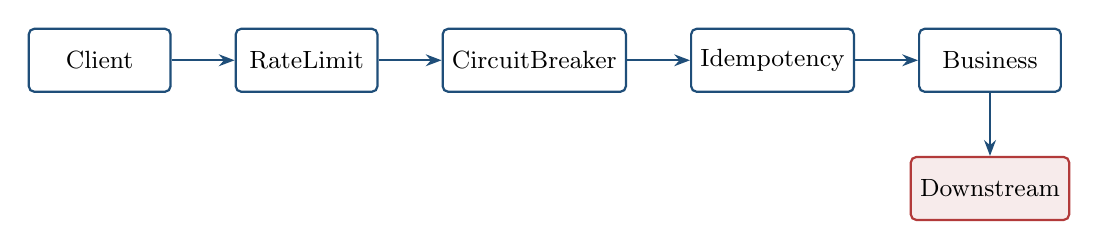
\begin{tikzpicture}[node distance=8mm and 8mm]
  \node[node-box] (cli) {Client};
  \node[node-box,right=of cli] (rl)  {RateLimit};
  \node[node-box,right=of rl] (cb)   {CircuitBreaker};
  \node[node-box,right=of cb] (id)   {Idempotency};
  \node[node-box,right=of id] (biz)  {Business};
  \node[node-box,below=of biz,node-bad] (down) {Downstream};
  \draw[arrow] (cli) -- (rl);
  \draw[arrow] (rl) -- (cb);
  \draw[arrow] (cb) -- (id);
  \draw[arrow] (id) -- (biz);
  \draw[arrow] (biz) -- (down);
\end{tikzpicture}
\vspace{2mm}
\begin{itemize}
  \item 限流在最外：阻挡总量。
  \item 熔断在中间：保护下游。
  \item 幂等在业务前：处理重复。
\end{itemize}
\end{frame}

\begin{frame}{熔断器单测：三态都 PASS}
\begin{tabular}{@{}lll@{}}
\toprule
用例 & 验证 & 结果 \\
\midrule
\texttt{OpensAfterFailures} & Closed $\to$ Open & PASS \\
\texttt{HalfOpenToClosed} & HalfOpen 全成功 $\to$ Closed & PASS \\
\texttt{HalfOpenFailReturnsToOpen} & HalfOpen 失败 $\to$ Open & PASS \\
\bottomrule
\end{tabular}
\vspace{3mm}
\srcnote{stressTest/REPORT.md 单元测试表 + middleware/circuitbreaker\_test.go}
\end{frame}

% ============== 5. 选型 ==============
\section{选型与边界}

\begin{frame}{选型决策树}
\begin{tabular}{@{}lll@{}}
\toprule
场景 & 工具 & 备注 \\
\midrule
单服务局部限流 & 令牌桶 (\texttt{x/time/rate}) & 内存内，毫秒级 \\
多实例全局限流 & Redis 滑动窗口 & 状态外置，精度高 \\
保护慢依赖 & 三态熔断器 & 关注失败率不是绝对值 \\
跨语言统一治理 & API Gateway / Sentinel & 业务侵入小 \\
\bottomrule
\end{tabular}
\vspace{3mm}
\keypoint{限流是\textbf{入口}治理，熔断是\textbf{出口}治理 —— 边界要分清。}
\end{frame}

% ============== Q&A ==============
\appendix

\begin{frame}{面试 Q\&A（上）}
\textbf{Q1}：令牌桶为什么允许"突发"？业务上需要吗？\\
\hspace{4mm}\small A：bucket capacity 给"短时尖峰"留缓冲，符合真实流量的脉冲特性。

\vspace{2mm}
\textbf{Q2}：单机限流 vs 分布式限流，分别用什么？\\
\hspace{4mm}\small A：单机用进程内令牌桶；多实例必须用 Redis 滑动窗口或令牌桶。

\vspace{2mm}
\textbf{Q3}：滑动窗口为什么用 ZSet 不用 List？\\
\hspace{4mm}\small A：ZSet 支持按 score 范围删 + O(1) 计数；List 只能按头尾，无法精确按时间清理。
\end{frame}

\begin{frame}{面试 Q\&A（下）}
\textbf{Q4}：熔断器的 half-open 探测请求数怎么选？\\
\hspace{4mm}\small A：3--5 个起步：太少噪声大，太多保护失效；按 P99 失败率反推。

\vspace{2mm}
\textbf{Q5}：限流后返回 429 还是 200+业务码？\\
\hspace{4mm}\small A：移动端为兼容老网关常用 200 + status=70001；标准 RESTful 用 429 +\texttt{Retry-After}。

\vspace{2mm}
\textbf{反追问}：限流值怎么设？\\
\hspace{4mm}\small A：压测找到 SLA 拐点 $\times$ 0.7，留余量；再按业务高峰 / 平峰区分。
\end{frame}

\begin{frame}{代码位置一览}
\begin{description}
  \item[令牌桶]\srcnote{middleware/ratelimit.go:22--49}
  \item[滑动窗口 mw]\srcnote{middleware/ratelimit.go:59--106}
  \item[滑动窗口 Lua]\srcnote{repository/cache/ratelimit.go:18--34}
  \item[熔断 allow]\srcnote{middleware/circuitbreaker.go:76--106}
  \item[熔断 report]\srcnote{middleware/circuitbreaker.go:108--128}
  \item[压测脚本]\srcnote{stressTest/seckill\_rate\_limit.js}
\end{description}
\vspace{2mm}
\keypoint{复现：\texttt{k6 run stressTest/seckill\_rate\_limit.js}}
\end{frame}

\end{document}
